\begin{figure}[H]
	\centering
	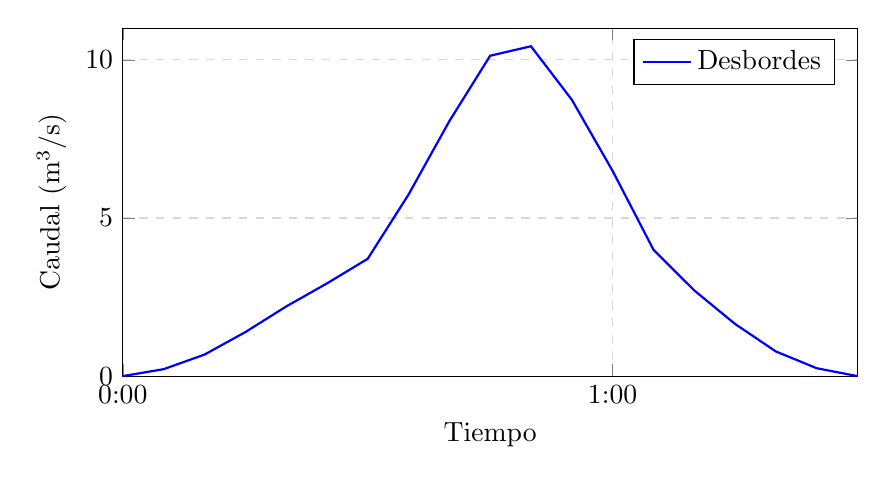
\begin{tikzpicture}
		\begin{axis}[
			width=0.9\textwidth,
			height=6cm,
			xlabel={Tiempo},
			ylabel={Caudal (m$^3$/s)},
			xmin=0,
			xmax=90,
			ymin=0,
			ymax=11,
			grid=major,
			grid style={dashed, gray!30},
			legend pos=north east,
			xtick={0, 60},
			xticklabels={0:00, 1:00},
			]
		% Desbordes
		\addplot [
		blue,
		thick,
		solid,
		] coordinates {
				(0, 0.00) (5, 0.22) (10, 0.68) (15, 1.39) (20, 2.20)
				(25, 2.93) (30, 3.71) (35, 5.74) (40, 8.06) (45, 10.13)
				(50, 10.43) (55, 8.74) (60, 6.49) (65, 4.00) (70, 2.71)
				(75, 1.65) (80, 0.78) (85, 0.25) (90, 0.00)
		};
		\addlegendentry{Desbordes}

		\end{axis}
	\end{tikzpicture}
	\caption{Hidrograma - Desbordes + BLOCKS $T_r$=10 años ($Q_p$=10.426 m$^3$/s)}
	\label{fig:hydro_desbordes_blocks_Tr10}
\end{figure}
